\section{Usage Examples}
\label{sec-usage}

This section presents six \PhoneLab{} usage examples. Each vignette begins by
highlighting an interesting or important aspect of the usage data we have
collected. Our goal, however, is not to conduct an exhaustive analysis.
Instead, each example continues by discussing how the presented results would
guide the design of future \PhoneLab{} experiments.

\subsection{Overall Battery Usage}
\label{subsec-batteryoverview}

\begin{figure*}[t]
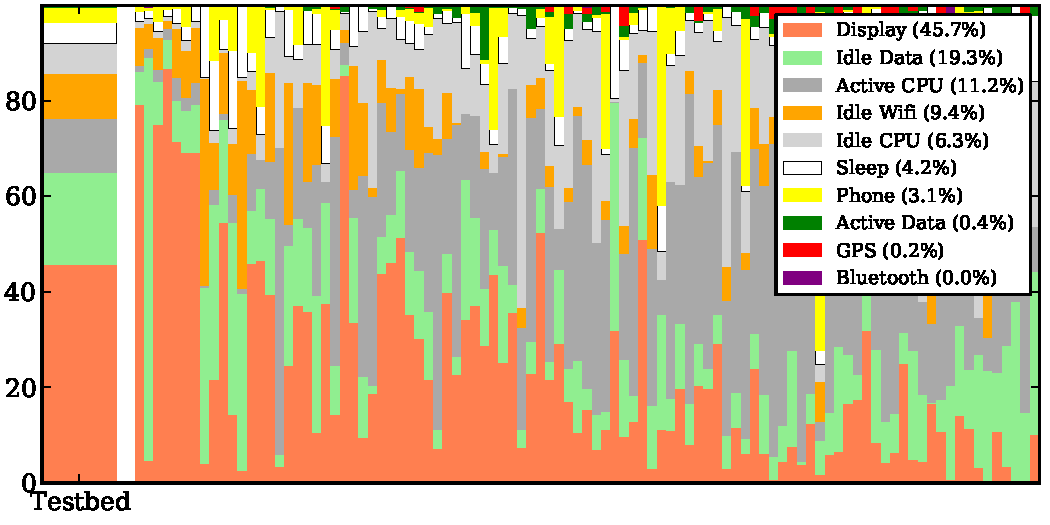
\includegraphics[width=\textwidth]{./figures/power/breakdown/graph.pdf}
\caption{Power usage by component.}
\end{figure*}

Smartphones are constrained by power, and a large amount of research on
smartphone systems is motivated by energy
conservation~\cite{FIXME,FIXME,FIXME}. While power is a definite concern,
evaluating the potential impact of energy saving approaches requires an
accurate breakdown of where energy is used by real phones. Only then can we
be sure we are addressing actual energy bottlenecks and use Amdahl's law to
put relative energy savings into context.

\subsubsection{Energy Breakdown}

\subsubsection{Future Experiments}

While previous smaller studies on earlier Android
models~\cite{shye:micro:2009} have presented similar taxonomies, the process
of identifying energy bottlenecks must be repeated regularly as hardware and
user behavior changes. \PhoneLab{} provides an ideal environment for
repeating energy usage experiments. Access to a stable set of participants
allows us to identify changes due to participant behavior, as participants
develop an awareness of the power consumption properties of their phones and
how to control them. And as we bring new hardware onto the testbed, we can
repeat power usage experiments to determine differences between smartphone
hardware generations.

